\documentclass[11pt]{article}
\usepackage{acl2016}
\usepackage{times}
% \usepackage[round]{natbib}
\usepackage{latexsym}
\usepackage[utf8]{inputenc}
\usepackage[font=small,labelfont=bf]{caption}
\usepackage{amsmath}
\usepackage{multirow}
\usepackage{appendix}
\usepackage{url}
\usepackage{tikz}
% \usepackage{avm}
% \avmfont{\sc}
% \avmoptions{sorted}
% \avmvalfont{\rm}
% \avmsortfont{\scriptsize\it}
\usepackage{remreset}
\usepackage{pifont}
% \newcommand{\cmark}{\ding{53}}%
\usepackage{graphicx}
\usepackage{wrapfig}
\usepackage{verbatim} 
\usepackage{linguex}
\usepackage{qtree}
%\usepackage{algorithm}% http://ctan.org/pkg/algorithms
%\usepackage{algpseudocode}% http://ctan.org/pkg/algorithmicx
\usepackage{amsmath,amsfonts,amssymb}

\newcommand{\argmax}{\operatornamewithlimits{argmax}}


\newcommand{\das}[1]{\emph{//das: #1//}}
\newcommand{\crk}[1]{\emph{//crk: #1//}}
\newcommand{\todo}[1]{\textcolor{green}{\emph{//todo: #1//}}}


\newcommand{\sds}[0]{\textsc{sds}}
\newcommand{\nlu}[0]{\textsc{nlu}}
\newcommand{\rmrs}[0]{\textsc{rmrs}}
\newcommand{\ep}[0]{\texttt{EP}}
\newcommand{\inprotk}[0]{\textsc{InproTK}}
\newcommand{\sium}[0]{\textsc{sium}}
\newcommand{\asr}[0]{\textsc{asr}}
\newcommand{\dm}[0]{\textsc{dm}}
\newcommand{\ui}[0]{\textsc{gui}}
\newcommand{\iu}[0]{\textsc{iu}}
\newcommand{\rr}[0]{\textsc{rr}}
\newcommand{\conf}[0]{\textsc{conf}}
\newcommand{\pa}[0]{\textsc{pa}}

%Document Head
% \dochead{CLV2 Class File Manual}

\title{An Adaptive, Incremental Personal Assistant that Graphically Signals Speech Understanding}

\author{Casey Kennington \and David Schlangen}
%\affil{CITEC, Bielefeld University}

% \author{David Schlangen}
% \affil{Bielefeld University}

\begin{document}
% \affil{Publishing / SPi}

\maketitle

% abstract should be 150-250 words
\begin{abstract}

\end{abstract}

\section{Introduction}
\label{section:intro}

Signaling understanding by backchannels is an essential aspect of spoken dialogue between humans and dialogue systems \cite{Yankelovich1995}. Humans signal understanding by providing feedback such as nodding, spoken backchannels (e.g., \emph{uh-huh}) or by performing some kind of action \cite{Clark1996}. Crucially, this feedback is provided as the utterance unfolds, such that installments of speech given by the speaker are confirmed as being understood before the speaker commits to continuing with speaking. Contrary to this, current virtual personal assistants (\pa s) require their users to either formulate complex intents in one utterance (as in ``make a phone call to Peter Miller on his mobile phone'') or go through tedious sub-dialogues (e.g., ``phone call'' -- \emph{who would you like to call?} -- ``Peter Miller'' -- \emph{I have a mobile number and a work number. Which one do you want?}). This is not how one would interact with a human assistant, where the request would be naturally structured into smaller chunks that individually get acknowledged (``Can you make a connection for me?'' -- \emph{sure} -- ``with Peter Miller'' - \emph{uh huh} - ``on his mobile'' - \emph{dialing now}). Current \pa s only signal ongoing understanding by displaying the state of the regonised speech (\asr) to the user, but simply recognising the speech does not denote understanding.\footnote{Suppose a native speaker of English is listening to and transcribing the speech of a native Spanish speaker with one important consideration: the native English speaker doesn't understand Spanish. Upon inspection, it could very well be the case that the transcription is somewhat accurate; the words are segmented properly and the spelling seems to mostly be correct. This illustrates the disconnect between speech reccognition (\asr) and natural language understanding (\nlu); i.e., \emph{intent recognition}: simply being able to recognise words is only the beginning of understanding speech.}

To address this, some \pa s attempt to learn a \emph{user model} so as to predict what it is the user wants from the system requiring little or no spoken input from the user. These can range on a continuum of \emph{non-predictive} systems that don't attempt to learn anything about the user, to \emph{fully-predictive} systems (such as Google Now) that attempt to predict what a user will utter before the user even utters it (e.g., a user receives a notification on her device with the text: \emph{Do you want to call Peter Miller?}). 

In this paper, we present a mixed graphical/voice enabled \pa\ that can provide feedback of understanding to the user \emph{incrmentally} as the user's utterance unfolds--allowing users to make requests in installments instead of fully thought-out requests. Our system does this by displaying ongoing understanding at each recognised word to the user in an intuitive tree-like graphical interface that can be displayed on a mobile devide. We evaluate our system by directing users to perform tasks using it under non-incremental (i.e., \asr\ endpointing) and incremental conditions and then asking the users to compare the two conditions with questionaires. We further compared the incremental version with a version that attempted to automatically predict the intent of the user based on that user's history. We report that the users found the interface intuitive and easy to understand, that the system could predict what they wanted, and that users were able to perform tasks more efficiently with incremental as well as adaptive variants of the system.

The remainder of this paper is organised as follows: in the following section, we provide a discussion of related work, then describe our system in Section~\ref{section:system_def}. We then explain the experiments and give the results in Section~\ref{section:experiments}. We then give a final discussion, ideas for future work, and conclude. 

\section{Related Work}
\label{section:related_work}

This work brings together and builds upon several threads of other previous research. \newcite{Chai2014} attempted to address misalignments in common ground \cite{clarkschaefer:contrdis} between systems (in their case, robots) and humans by informing the human of the internal state of the system (through speech from the robot). We take this idea and apply it to a \pa\ by displaying the internal state of the system to the user in an intuitive, tree-like structure (explained in Section~\ref{section:display}), allowing the user to determine if understanding has taken place by the system. Such information presentation is a way of providing feedback and backchannels to the user. \newcite{Dethlefs2015} provides a good review of work that shows that backchannels facilitate grounding, feedback, and clarifications in human spoken dialogue, and apply an \emph{information density} approach to determining when to backchannel using speech. Because we don't backchannel using speech here, there is no potential overlap between the human user and the system; rather, our system can display backchannels and ask clarifications without interrupting (that is, frustrating) the user. 

Though different in many ways, our work is similar in some regards to \newcite{Larsson2011}, which displays information to the user and allows the user to navigate the display itself (e.g., by saying \emph{up} or \emph{down} in a menu list)--functionality that we intend to apply to our display in future work. 

Some of the work here is inspired by the \emph{Microsoft Language Understanding Intelligent Service} (LUIS) project \cite{Williams2015_sigdial}. While our system by no means achieves the scale that LUIS does, we offer here an open source LUIS-like system (with the important addition of the graphical interface) that is authorable (using JSON files; we leave authoring using a web interface--like LUIS--to future work), extendible (affordances can be easily added), incremental (going beyond LUIS), trainable (i.e,. can learn from examples, but can still function well without examples), and can learn through interacting (here we apply a simplified user model that learns during interaction). 

\section{System Description}
\label{section:system_def}

This section introduces and describes our \sds, which is modularised into four main components: automatic speech recognition (\asr), natural langauge understanding (\nlu), dialogue management (\dm), and the user interface (\ui) which, as explained below, is visualised as a right-branching tree. The overall system is represented in Figure~\ref{fig:overview}. For the remainder of this section, each module is exlpained in turn. As each module processes input incrementally (i.e., word for word), we first explain our framework for incremental processing.

\begin{figure}[ht]
  \centering
      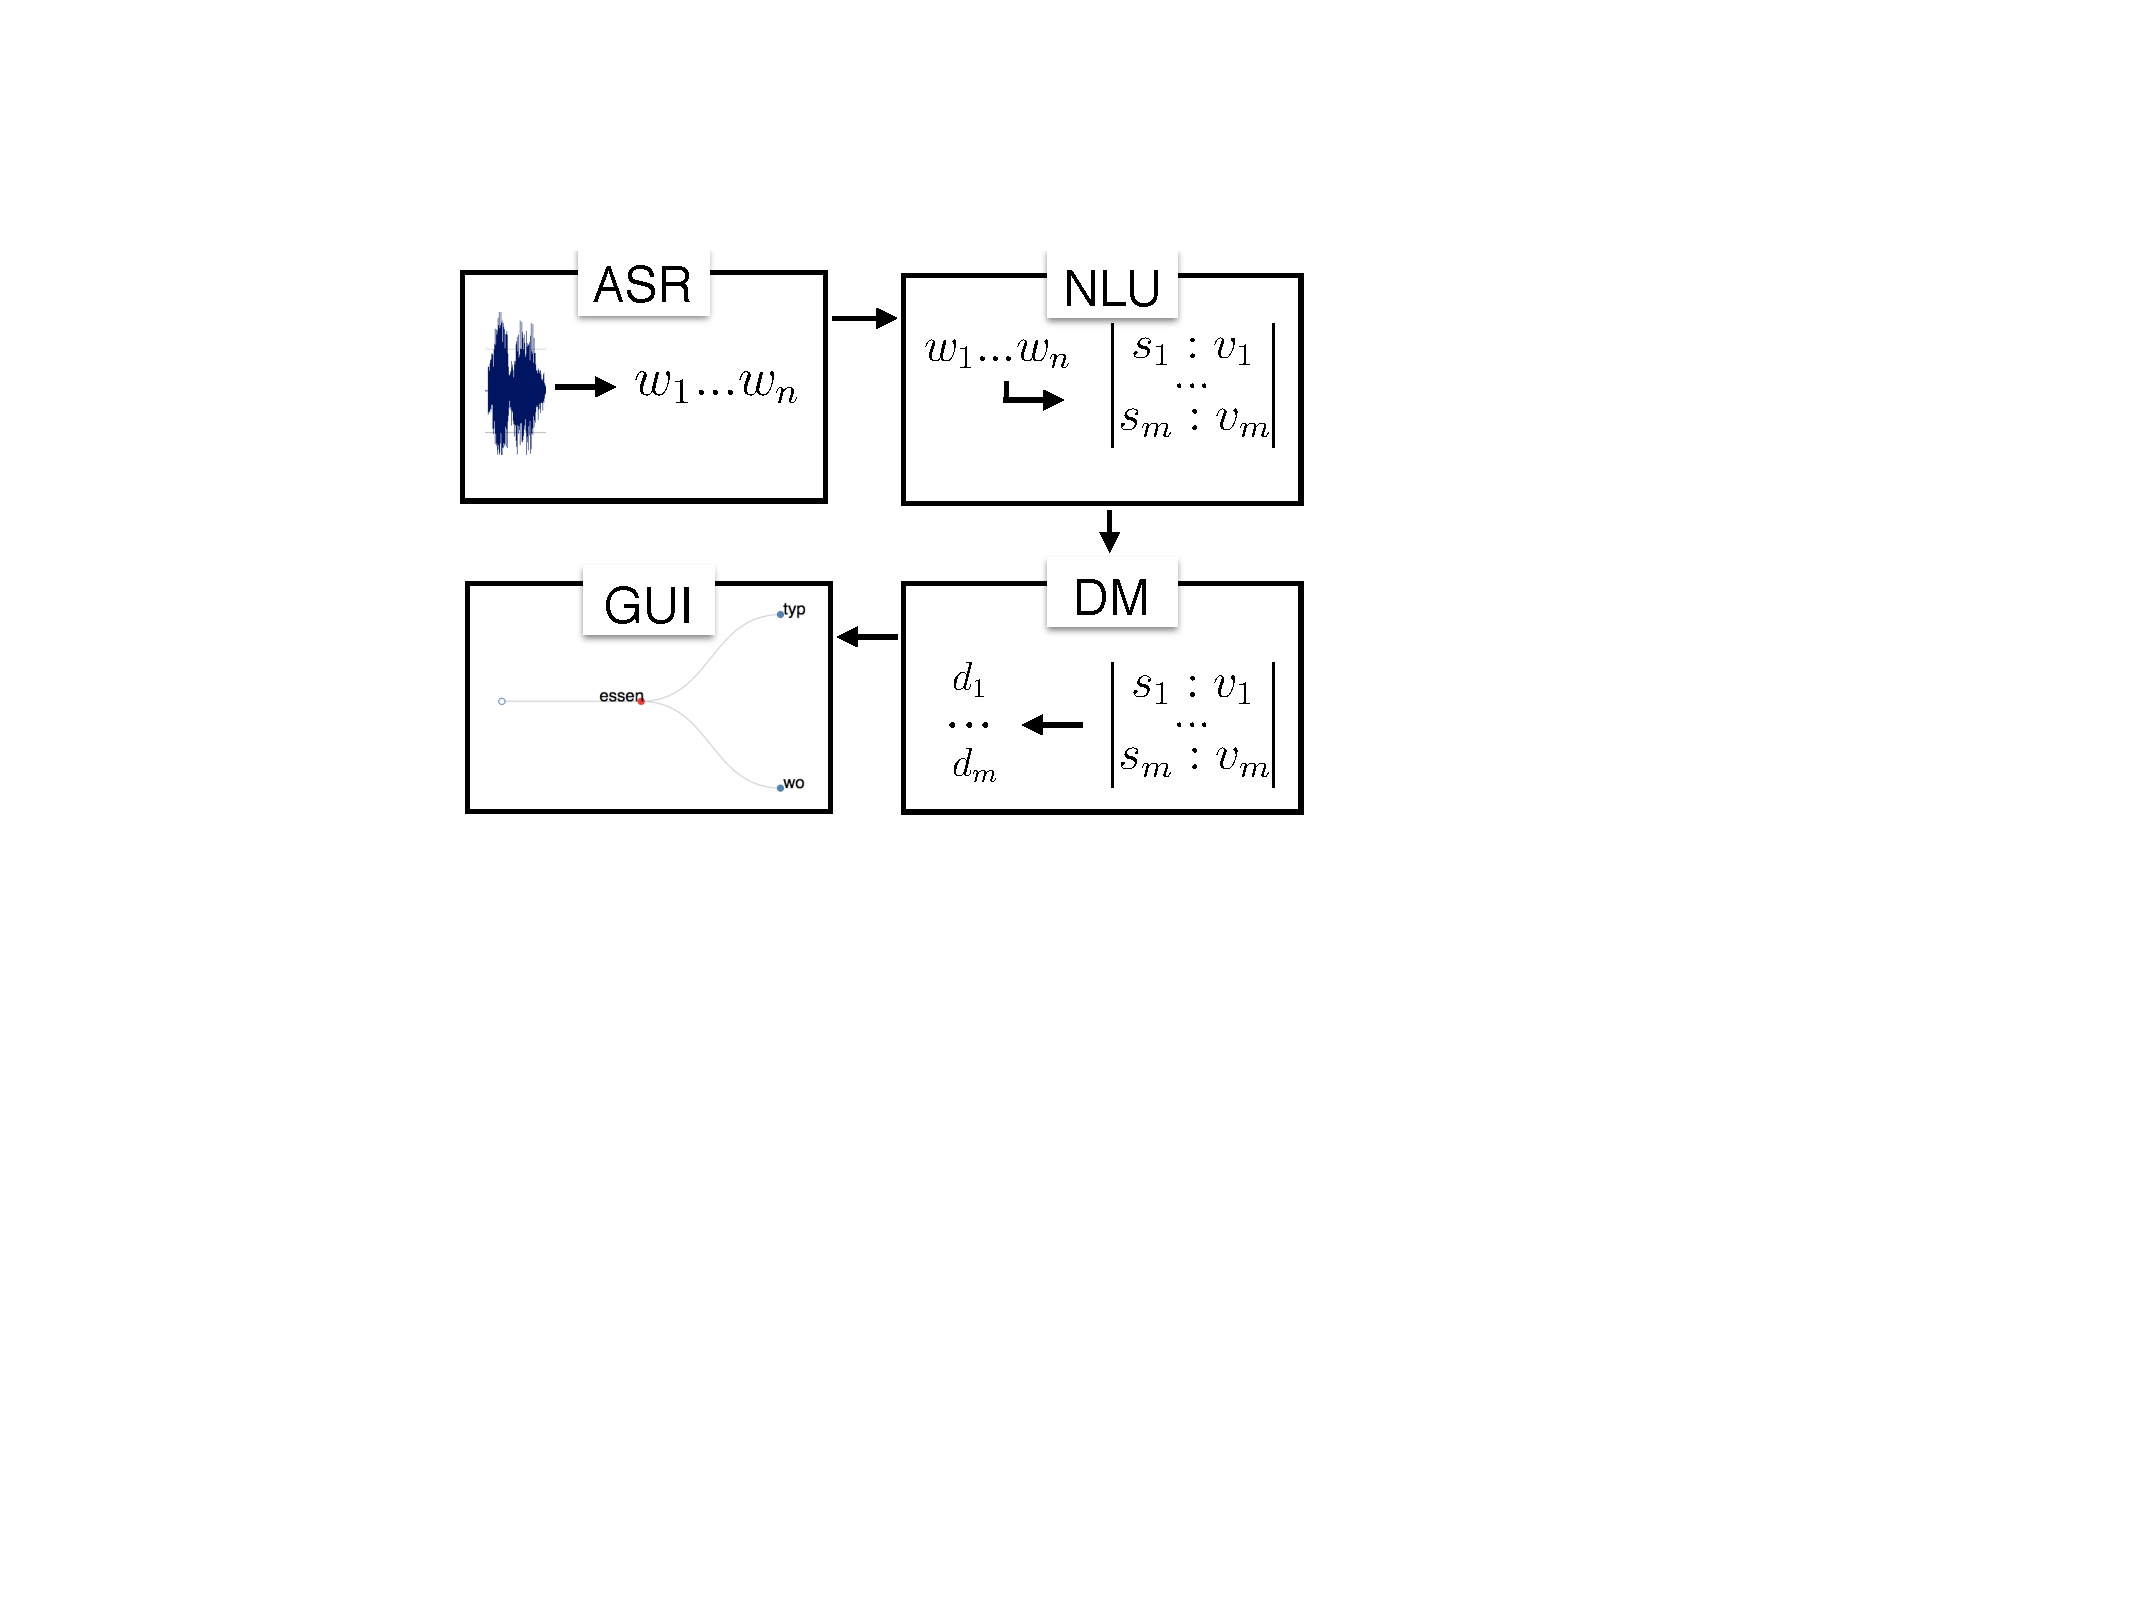
\includegraphics[width=0.5\textwidth]{figures/sig16-overview.pdf}	
      \caption{Overview of system made up of \asr\ which takes in a speech signal and produces transcribed words, \nlu, which takes words and produces a slots in a frame, \dm\ which takes slots and produces a decision for each, and the \ui\ which displays the state of the system. \label{fig:overview}}
\end{figure}


\subsection{Incremental Dialogue}

Of prime importance in our \sds--an aspect of our \sds\ that sets it apart from others--is the requirement that it processes \emph{incrementally}. An often-cited concern with incremental processing is regarding informativeness: why act early when waiting (even just for a moment) would allow additional information, resutling in more-informed decisions? The trade-off here is all-important: \emph{naturalness} as perceived by the end user who is interacting with the \sds. Indeed, it has been shown that humans perceive incremental systems as being more natural than traditional, turn-based systems \cite{Aist2006,Skantze2009,skantze2010sigdial,Asri2014}, offer a more human-like experience for the human users \cite{Edlund2008b} and are more satisfying to interact with than non-incremental systems \cite{Aistetal:incrunder-short}. Psycholinguistic research has also shown that humans process (i.e., comprehend) utterances as they unfold and do not wait until the end of an utterance to begin the comprehension process \cite{Tanenhaus1995,Spivey_2002tw}. 

The trade-off between informativeness and naturalness can be reconciled when mechanisms are in place where earlier desicions can be repaired. Such mechanisms were introduced in the incremental unit (\iu) framework for \sds\ \cite{Schlangen2011}, which we apply here. Following \newcite{kennington-kousidis-schlangen:2014:W14-43}, incremental systems consist of a network of processing \emph{modules}. A typical module takes input from its \emph{left buffer}, performs some kind of processing on that data, and places the processed result onto its \emph{right buffer}. The data are packaged as the payload of \emph{incremental units} (\textsc{iu}s) which are passed between modules. The \textsc{iu}s themselves are interconnected via so-called \emph{same level links} (\textsc{sll}) and \emph{grounded-in links} (\textsc{grin}), the former allowing the linking of \textsc{iu}s as a growing sequence, the latter allowing that sequence to convey what \textsc{iu}s directly affect it (see Figure \ref{fig:iu_example} for an example of incremental \asr). Thus \iu s can be \emph{added}, but can be later \emph{revoked} and replaced in light of new information. This allows incremental components to take advantage of up-to-date information, but have the potential to function in such a way that users perceive the system as more natural.

\begin{figure} %[ht]
  \centering
      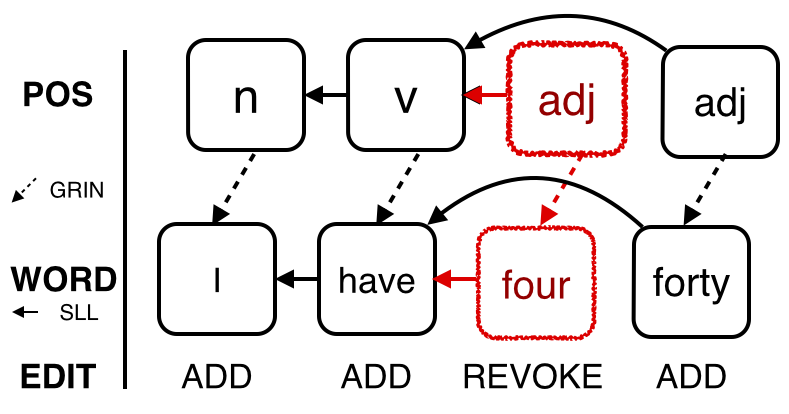
\includegraphics[width=0.45\textwidth]{figures/005_iu_example.png}	
      \caption{Example of IU network; part-of-speech tags are grounded into words, tags and words have same level links with left IU; \emph{four} is revoked and replaced with \emph{forty}.\label{fig:iu_example}}
            \vspace{-0.25cm}
\end{figure}

The modules exlpained in the remainer of this section are implemented as \iu-modules and process incrementally. Each will now be explained. 

\subsection{Speech Recognition}

In the case of our \sds, the module that takes speech input from the user is the \asr\ component. Incremental \asr\ must transcribe uttered speech into words and words must be forthcoming from the \asr\ as early as possible (i.e., the \asr\ must not wait for endponiting in order to act). Each module that follows must also process incrementally, acting in lock-step upon input as it is received. Incremental \asr\ is not new \cite{baumannetal2009:naacl} and many of the current freely-accessible \asr\ systems can produce output (semi-) incrementally. 

In our \sds, we opt for Google \asr\ because of its wide vocbaulary coverage of the language we are evaluating in (German). We are able to package \asr\ output from the Google service into \iu s as explained above. Those word \iu s are passed to the \nlu\ module, which will now be explained. 

\subsection{Language Understanding}

We approach the task of \nlu\ as a slot-filling task (a very common approach; see \newcite{Tur2012}) where an intent is complete when all slots of a \emph{frame} are filled. The main driver of the \nlu\ in our \sds\ is the \sium\ model of \nlu\ introduced in \newcite{Kennington2013a}. \sium\ has been used in several systems which have reported impressive results in various domains, languages, and tasks \cite{Kennington2014_coling,Kennington2015_naacl}. Though originally a model of reference resolution, the authors hinted that it could be used for general \nlu, which we do here. The model is formalised as follows:

\begin{center}
\begin{equation}
   P(I|U) = \frac{1}{P(U)} P(I)\sum_{r\in R} P(U|R)P(R|I) 
\label{eq:disc1}
\end{equation}
\end{center}

That is, $P(I|U)$ is the probability of the intent $I$ (i.e., a frame slot) behind the speaker's (ongoing) utterance $U$. This is recovered using the mediating variable $R$, a set of \emph{properties} which map between aspects of $U$ and aspects of $I$. We opt for abstract properties here (e.g., the intent of a \texttt{restaurant} might be filled by a certiain type of cusine such as \texttt{italian} which has, among others, properties like \texttt{pasta}, \texttt{mediteranian}, \texttt{vegetarian}, etc.). Properties are pre-defined by a system designer and can match words that might be uttered to describe the intent in question. The mapping betwen properties and aspects of $U$ can be learned from data. During application, $P(U|R)$ can produce a distribution over words which are summed over and the probability mass for each property is accumulated for each intent, resulting in a distribution over possible intents.\footnote{In \newcite{Kennington2013a} the authors apply Bayes' Rule to allow $P(U|R)$ to produce a distribution over properties, which we adopt here.} This occurs at each word increment, where the distribution from the previous increment is combined via $P(I)$, keeping track of the distribution over time. 

To allow our system to function with minimal amounts of training data, we apply a simple rule: if some $r \in R$ and $w \in U$ are such that $r=w$ (e.g., an intent has the property of \texttt{pasta} and the word \emph{pasta} is uttered, then $P(U=w|R=r) = 1$.

In our \sds, we apply an instantion of \sium\ for each slot, all of which update at each word increment. At each word increment, the updated slots (and their corresponding) distributions are given to the \dm, which will now be explained. 

\subsection{Dialogue Manager}

The primary job of our \dm\ is to determine \emph{when} to act, given the unfolding utterance. That is, at each word, the \dm\ needs to choose one of the following:
\begin{itemize}
 \item \texttt{wait} -- don't act until more information is forthcoming
 \item \texttt{select} -- the \nlu\ is confident enough that a slot can be filled with the argmax for this slot from \nlu.
 \item \texttt{request} -- the dialogue has reached a state where the system has asked for a (yes/no) clarification request
 \item \texttt{confirm} -- the user has responded to the clarification request (which acts similar to a \texttt{select})
\end{itemize}

This is a crucial part to our \sds\ which sets it apart from other systems in that the \dm\ is called upon at each word to decide \emph{when} to act, rather than \emph{how} to act, effecively giving the \dm\ the control over timing of actions rather than relying on \asr\ endpointing. The \dm\ policy is based on a confidence score (\conf) derived from the \nlu\ (in this case, we used the distribution's argmax value) using thresholds for \texttt{wait}, \texttt{confirm} and \texttt{select} set by hand (i.e., trial and error). Though the thresholds were statically set, we applied OpenDial \cite{Lison2015a} as an \iu-module to perform the task of the \dm\ with the future goal that these values could be adjusted through reinforcement learning (which OpenDial could provide). The \dm\ processes and makes a decision for \emph{each slot}, with the assumption that only one slot out of all that are processed will result in an non-\texttt{wait} action (though this is not constrained). The candidate slots that are processed depends on the state of the \ui\ (described below); only slots represented by visible nodes are considered, thereby reducing the possible frames that could be predicted.

\subsection{Graphical User Interface}
\label{section:display}

The goal of the \ui\ is to inform the user about the internal state of the ongoing understanding. One motivation for this is that the user can determine if the system understood the user's intent before providing the user with a response (e.g., a list of restaurants of a certain type); i.e., if any misunderstanding takes place, it happens before the system commits to an action and is potentially more easily repaired. 

\begin{wrapfigure}{r}{0.25\textwidth}
  \centering
      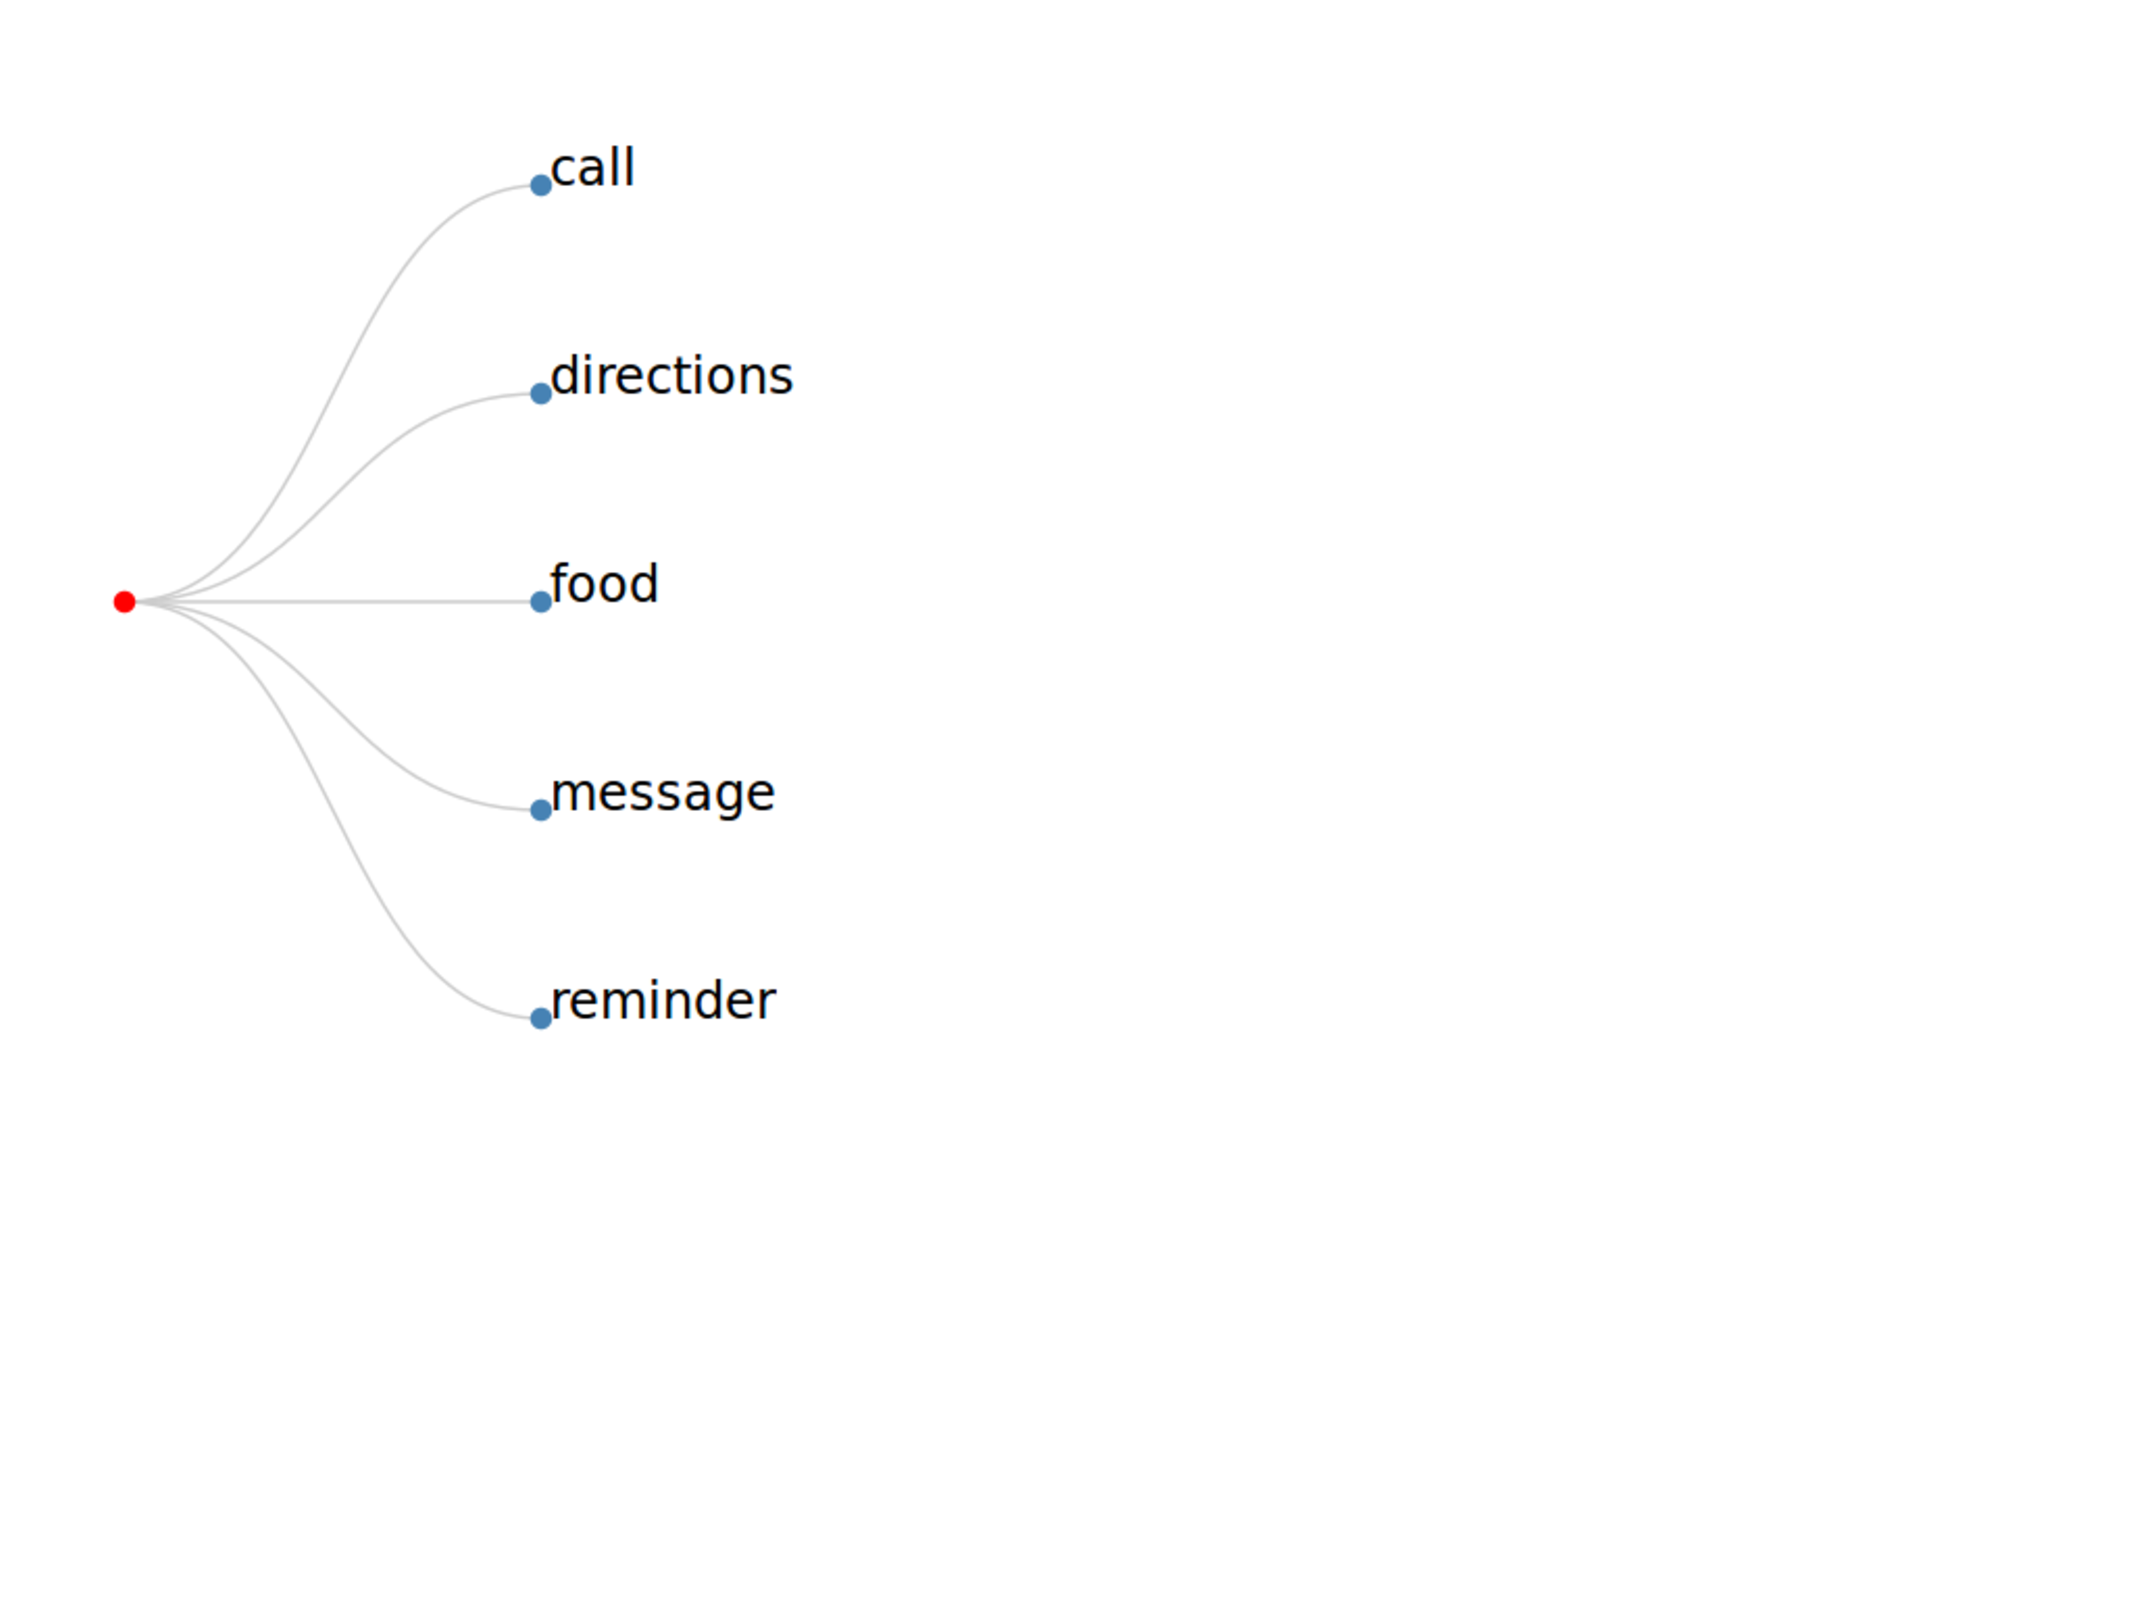
\includegraphics[width=0.25\textwidth]{figures/diatree-affordances.pdf}	
      \caption{Example tree as branching from the root; each branch represents a system affordance (i.e., making a phone call, reminder, finding a restaurant, leaving a message, and finding a route). \label{fig:afforances}}
\end{wrapfigure}

The display is a right-branching tree, where the branches directly off the root node display the afforances of the system (i.e., what domains of things it can understand and do something about). When the first tree is displayed, it represents a state of the \nlu\ where none of the slots are filled, an example of which is shown in Figure~\ref{fig:afforances}. 

When a user selects a domain to ask about, the tree is adjusted to make that domain the only one displayed and the slots that are required for that domain are shown as branches. The user can then fill those slots (i.e., branches) by uttering the name of the slot, or, alternatively, by uttering the item to fill the slot directly. For example, at a minimum, the user could utter the name of the domain then an item for each slot (e.g.,  \emph{food Thai downtown}) or the speech could be more natural (e.g., \emph{I'm quite hungry, I am looking for some Thai food maybe in the downtown area}). When something is uttered that falls into the \texttt{request} state of the \dm\ as explained above, the display expands the subtree under question (\todo{bring QUD into this?}) and marks the item with a question mark (see Figure~\ref{fig:confirm}). At this point, the user can utter any kind of confirmation. A positive confirmation would fill the slot with the item in question, collapsing that particular branch of the tree. A negative confirmation would retract the question, but leave the branch expanded. The expanded branches are displayed according to their rank as given by the \nlu's probability distribution. Though a branch in the display can theoretically display an unlimited number of children, we opted to only show as many as 7 children; if a branch had more than 7 children, the final (bottom-most) child was an ellipsis. 

\begin{figure}[ht]
  \centering
      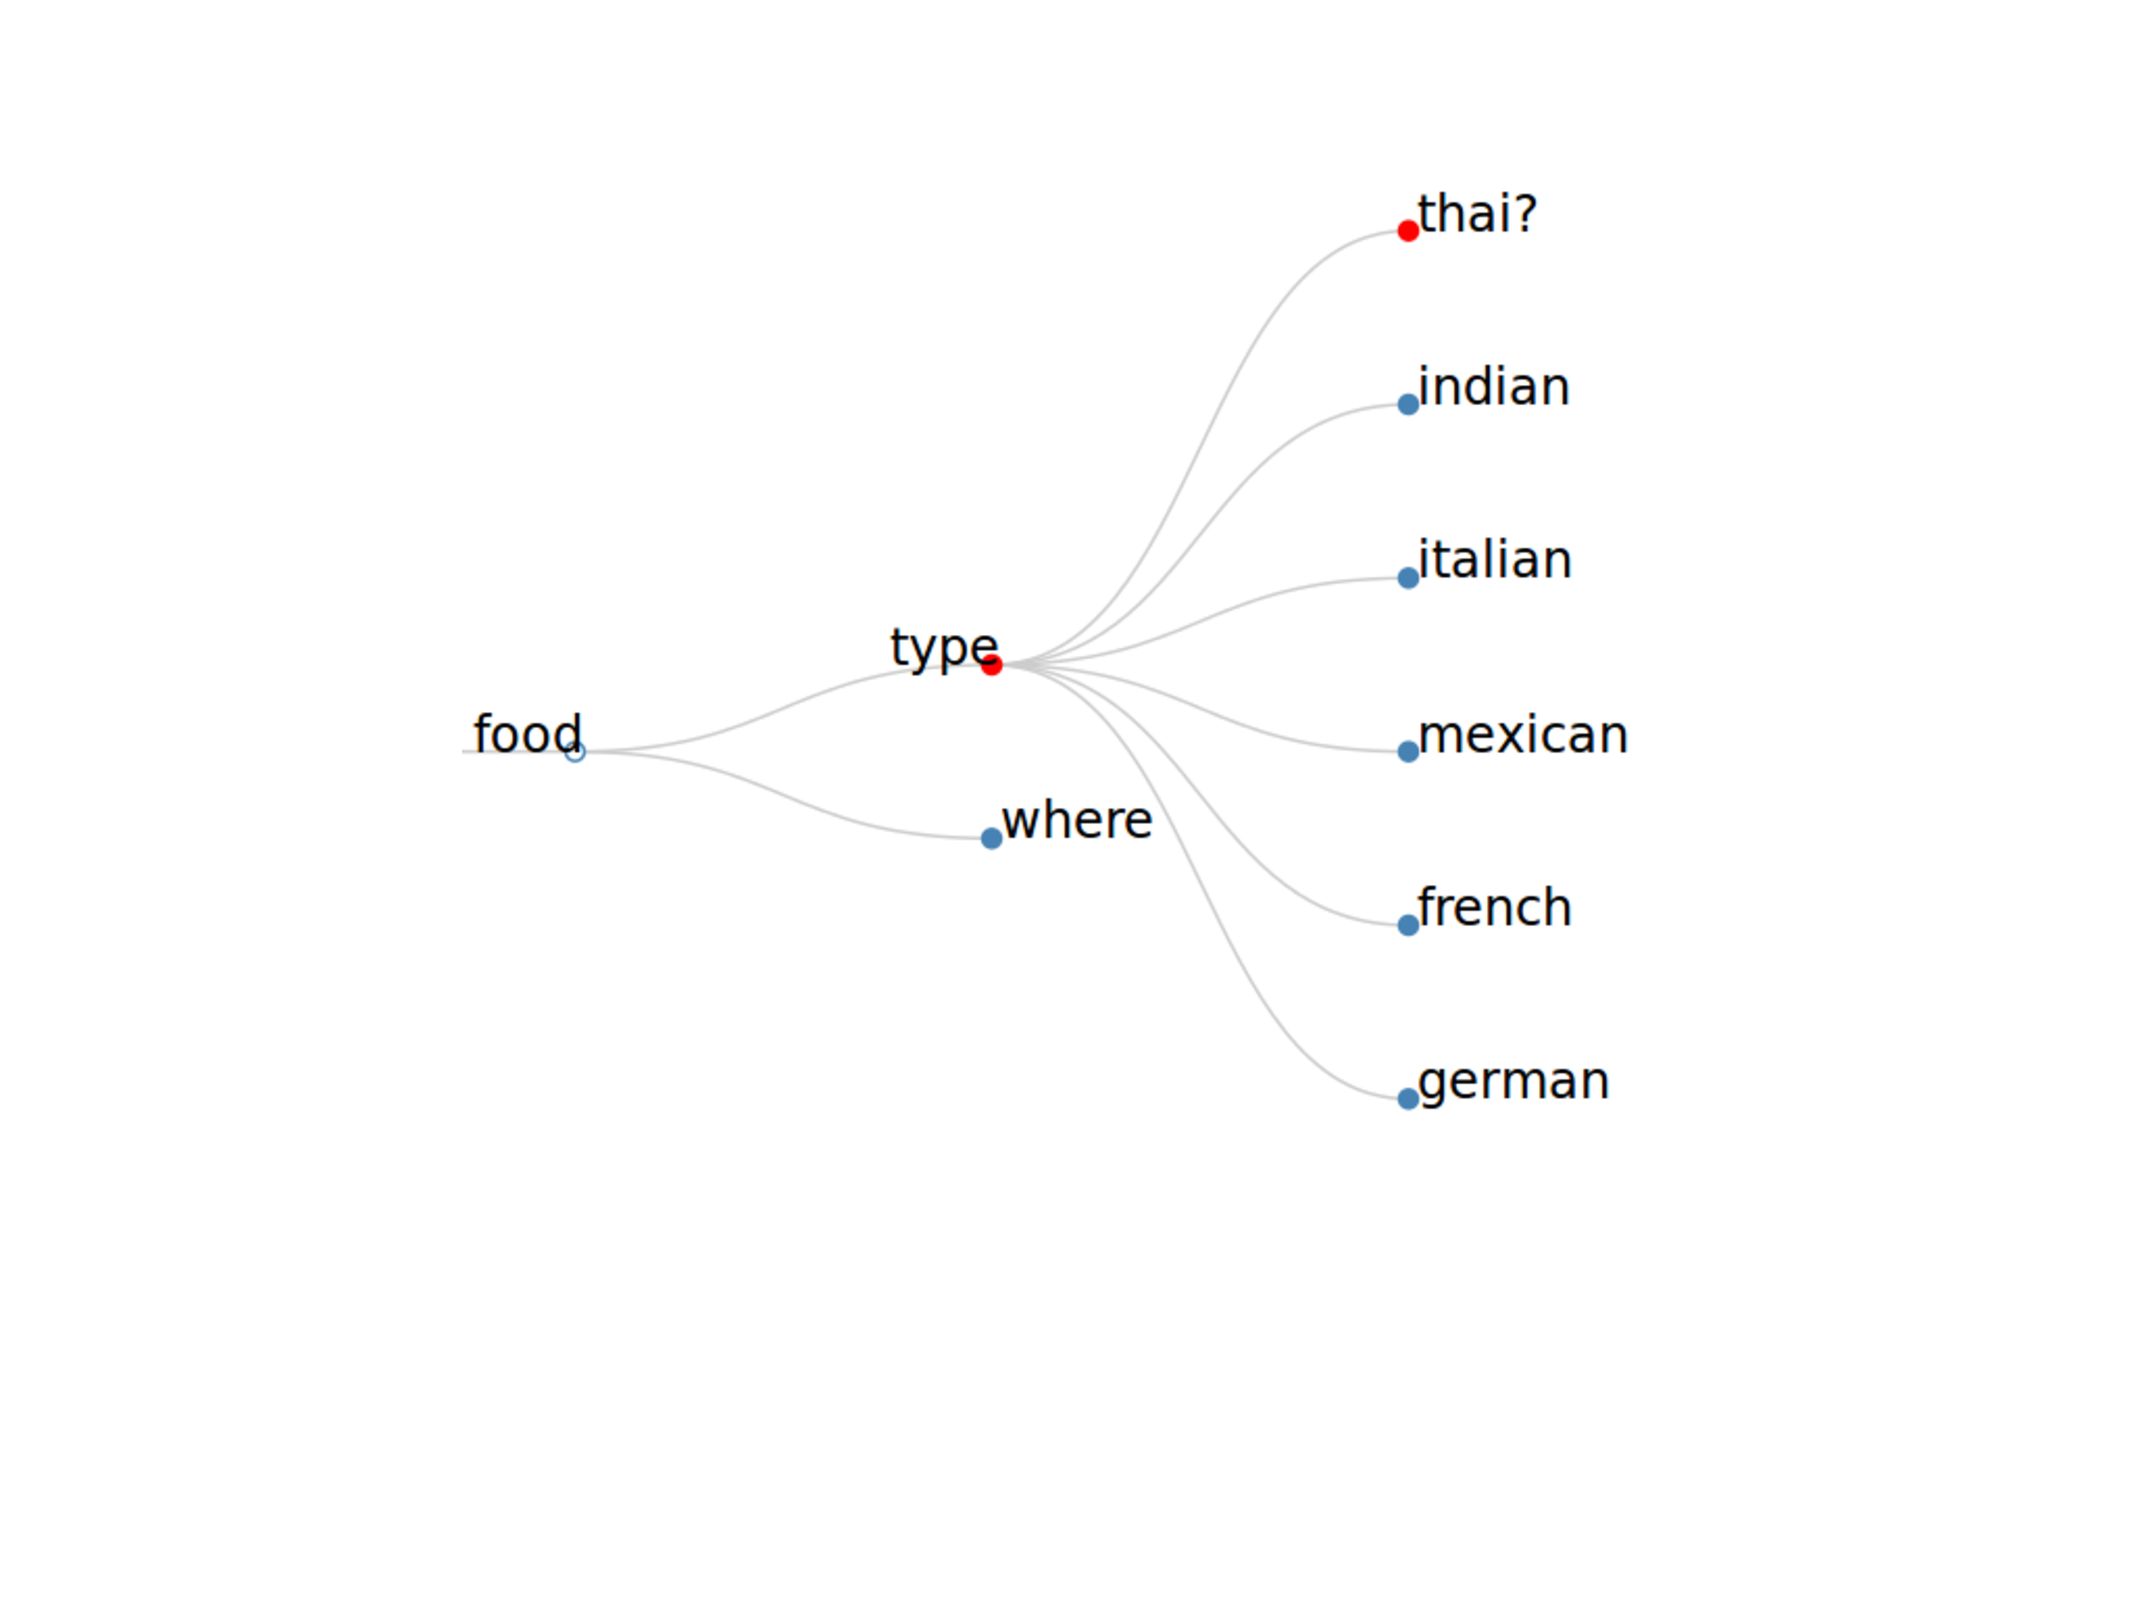
\includegraphics[width=0.5\textwidth]{figures/diatree-confirmation.pdf}	
      \caption{Example tree asking for confirmation on a specific node (in red with a question mark).\label{fig:confirm}}
\end{figure}

A filled  branch is collapsed, visually marking its corresponding slot as filled. At any time, a user can backtrack by saying \emph{no} (or equivalent) or start the entire interaction over from the beginning with a keyword, e.g., \emph{restart}. To aid the user's attention, the node under question is marked in red, where filled slots are represnted by blue nodes, and filled nodes represent candidates for the current slot in question. For cases where the system is in the \texttt{wait} state for several words (during which there is no change in the tree), the system signals activity at each word by causing the red node in question to temporarily change to white, then back to red (i.e., appearing as a blinking node to the user). Figure~\ref{fig:filled} shows a completeld filled frame, represented as tree with one branch for each filled slot.

\begin{figure}[ht]
  \centering
      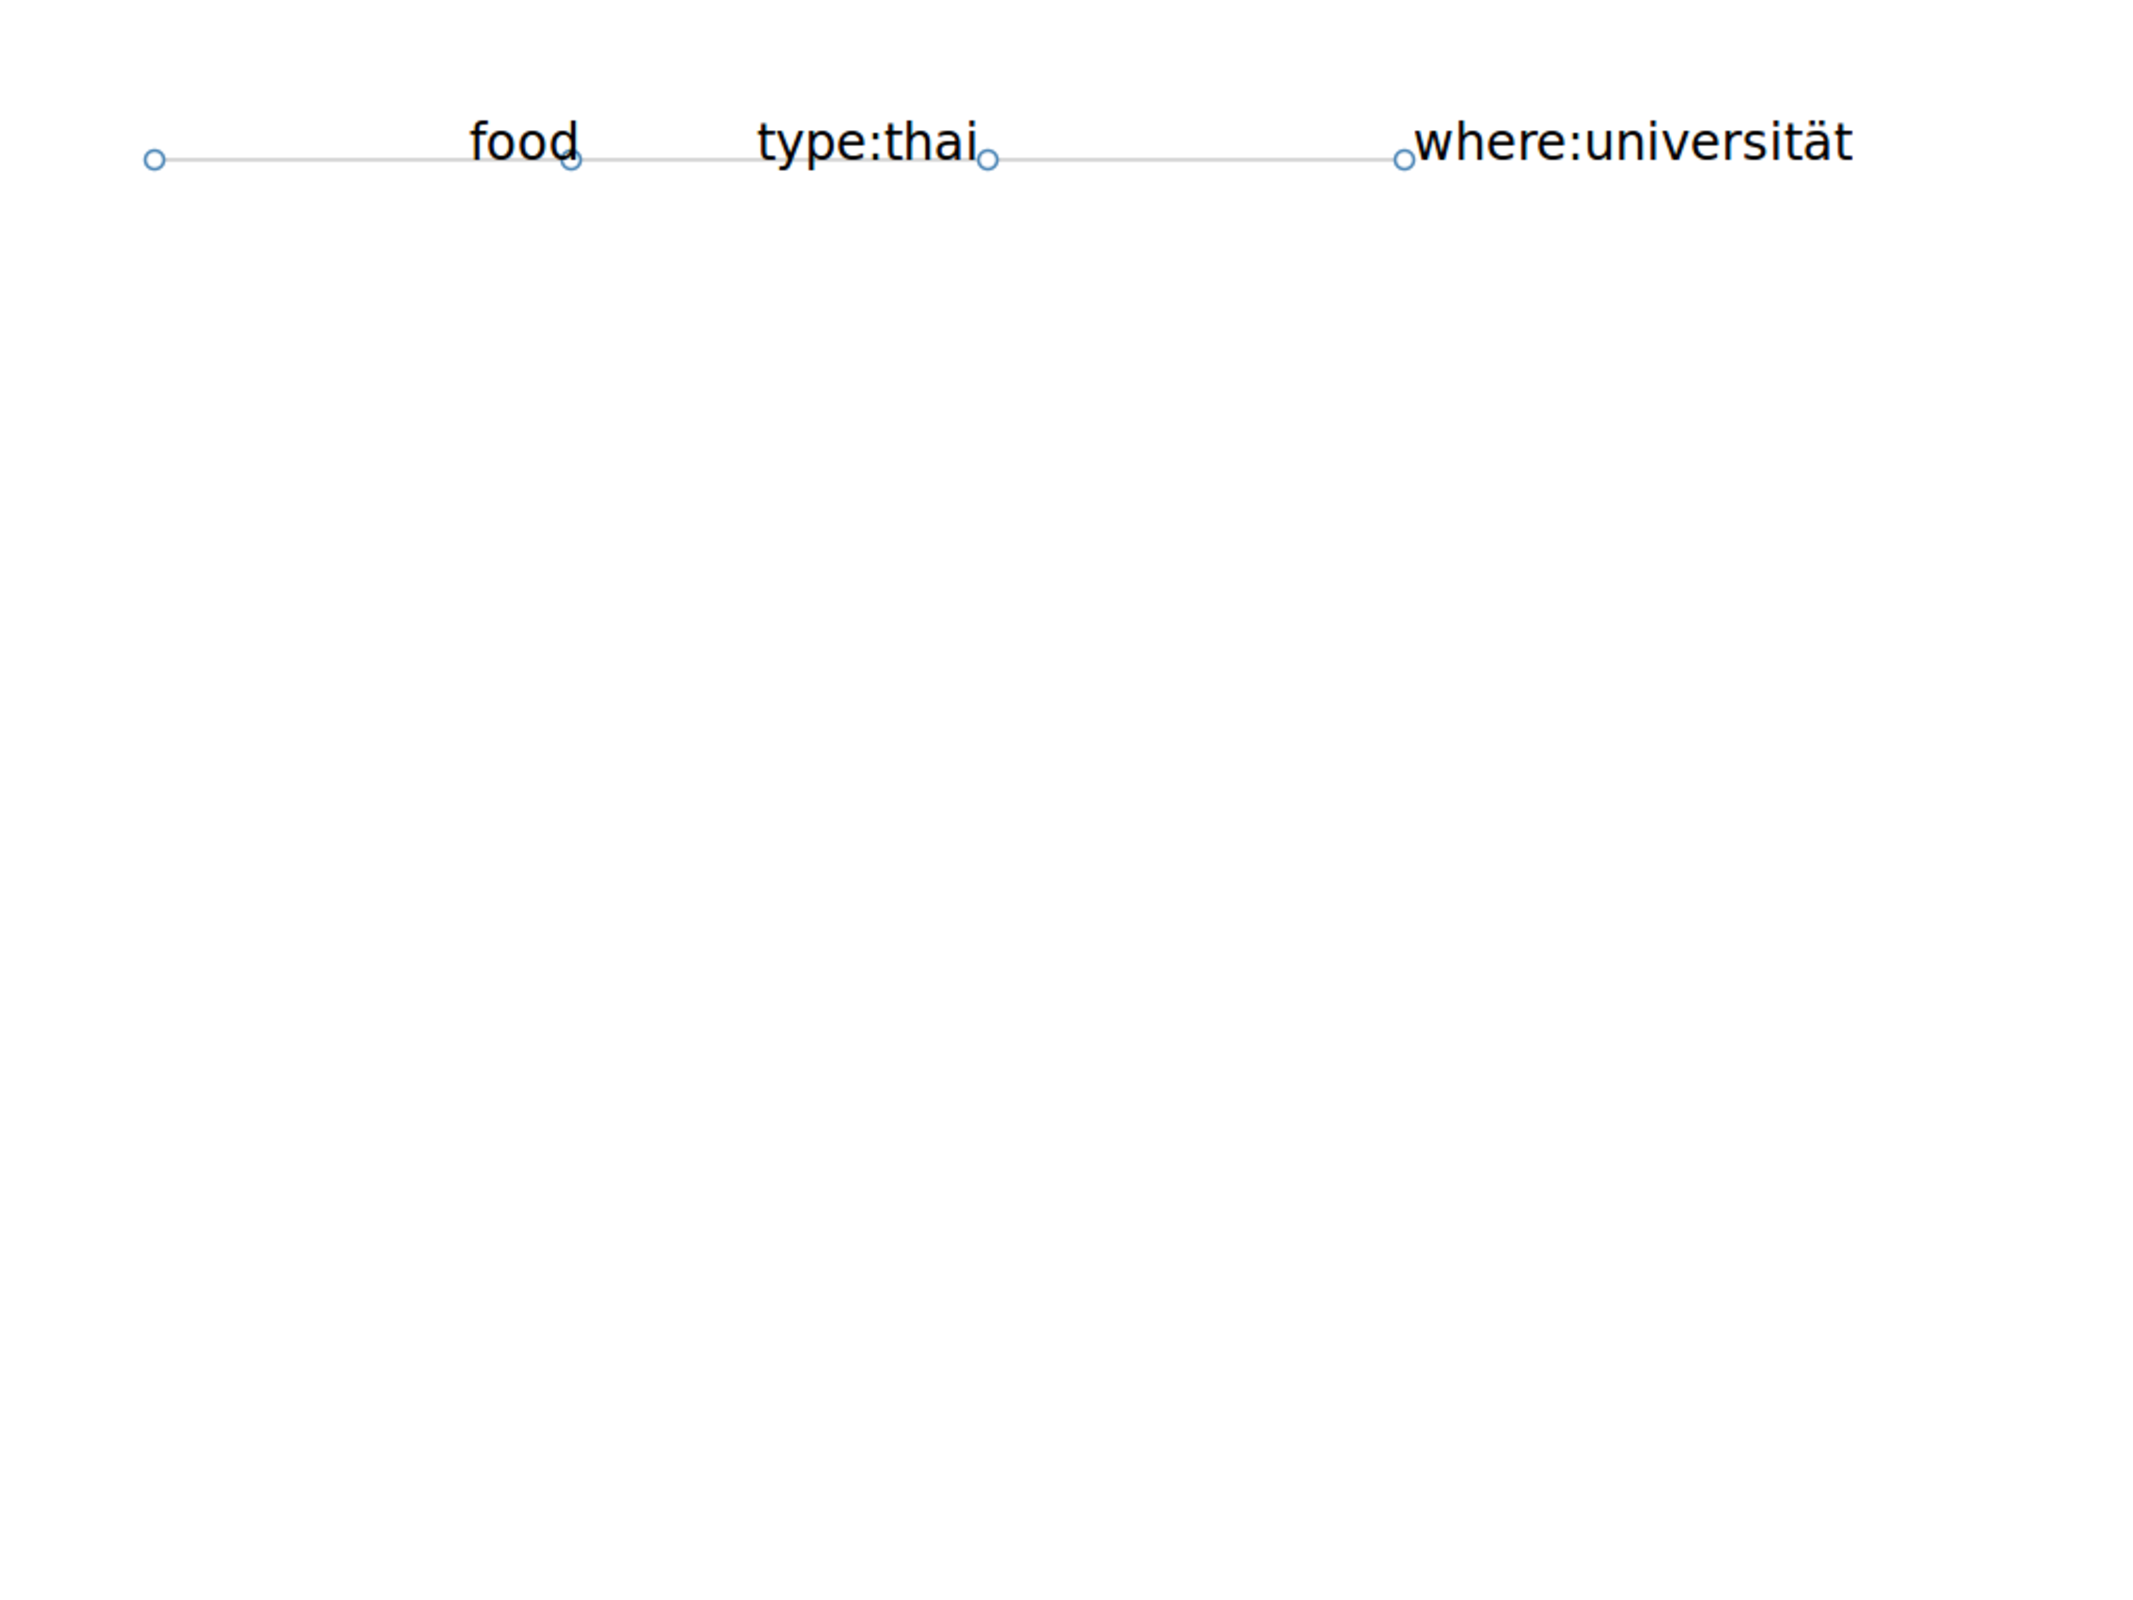
\includegraphics[width=0.5\textwidth]{figures/diatree-filled.pdf}	
      \caption{Example tree where all of the slots are filled. (i.e., \texttt{domain:food}, \texttt{location:nearby}, \texttt{type:french}) \label{fig:filled}}
\end{figure}

Such an interface clearly shows the internal state of the \sds\ and whether or not it has understood the request so far. It is desinged to aid the user's attention to the slot in question, and clearly indicates the affordances that the system has. The interface is currently a read-only display that is purely speech-driven, but it could be augmented with additional funcionalities, such as tapping a node for expansion or typing intput that the system might not yet display. It is currently implemented as a web-based interface (using the javascript D3 library), allowing it to be usable as a web application on any machine or mobile device. 


\section{Experiments}
\label{section:experiments}

In this section, we describe two experiments in which we evaluated our system. It is our primary goal to show that our \ui\ is useful to the user and signals understanding to the users. We also desire to show that incremental presentation of such a \ui\ is more effective than an endpointed system. We further want to show that an adaptive system is more effective than a non-adpative system (though both would process incrementally). In order to best evaluate our system, we recruited participants to interact with our system in varied settings to compare endpointed (i.e., non-incremental) and incremental as well as adaptive (also incremental) versions. We will describe how the data were collected from the participants, then explain each experiment and give results.

\subsection{Task \& Procedure} 


\begin{wrapfigure}{r}{0.3\textwidth}
  \centering
      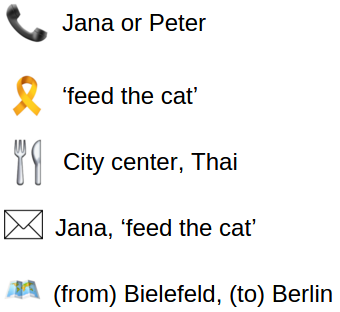
\includegraphics[width=0.3\textwidth]{figures/taskexample.png}	
      \caption{Examples of tasks, as presented to each participant. Each icon represents a specific task domain (i.e., call, reminder, find a restaurant, leave a message, or directions).\label{fig:taskex}}
\end{wrapfigure}

The participants were seated at a desk and given written instructions indicating that they were to use the system to perform as many tasks as possible in the allotted time. The instructions gave them several examples of kinds of tasks the system could understand with an icon representing the domain and then text for the rest of the task, as shown in Figure~\ref{fig:taskex}. In front of the participant towards the rear of the table was a computer screen that would show the task in the middle of the screen. In front of that screen closer to the participant was a small tablet that showed the \ui.\footnote{We used a Samsung 8.4 Pro turned to its side to show a larger width for the tree to grow to the right.} The user was instructed to convey the task presented on the screen to the system such that the \ui\ on the tablet would have a completed tree (i.e., the tree was in its filled state as in Figure~\ref{fig:filled}). When the participant was satisfied that the system understood her intent, she was to press spacebar on a keyboard in front of the tablet which triggered a new task to be displayed and the screen and reset the tree to its start state on the tablet (which was the root node linking to the 5 possible tasks). See Figure~\ref{fig:dataview} for an overview of the experiment setup.


The possible tasks were \emph{call}, which had a single slot for \emph{name} to be filled (i.e., one out of the 22 most common German given names); \emph{message} which had a slot for \emph{name} and a slot for the \emph{message} (which, when invoked, would simply fill in directly from the \asr\ until 1 second of silence was detected); \emph{eat} which had slots for \emph{type} (in this case, 6 possible types) and \emph{location} (in this case, 6 possible known locations based around the city of Bielefeld); \emph{route} which had slots for \emph{source} city and the \emph{destination} city; and \emph{reminder} which had a slot for \emph{message}. Some of the slot types were shared across domains, such as \emph{message} (across \emph{reminder} and \emph{message}), \emph{name} (across \emph{message} and \emph{call}), as well as \emph{source} and \emph{destination} which shared the same list of German city names (the top 100 most populous cities). 



The tasks presented to the participant were randomly chosen: first, the domain was randomly chosen from the 5 possible domains, and then each slot value to be filled was randomly chosen (the \emph{message} slot for the \emph{name} and \emph{message} domains was randomly selected from a list of 6 possible ``messages'', each with 2-3 words; e.g., \emph{feed the cat}, \emph{visit grandma}, etc.). The system kept track of which tasks were already presented to the participant. At any time after the first task, the system could choose a task that was previously presented and present it again to the participant (with a 50\% chance) so the user would often see tasks that she had seen before (with the assumption that humans who use \pa s often do perform similar, if not the same, tasks more than once). 

\begin{figure}[ht]
  \centering
      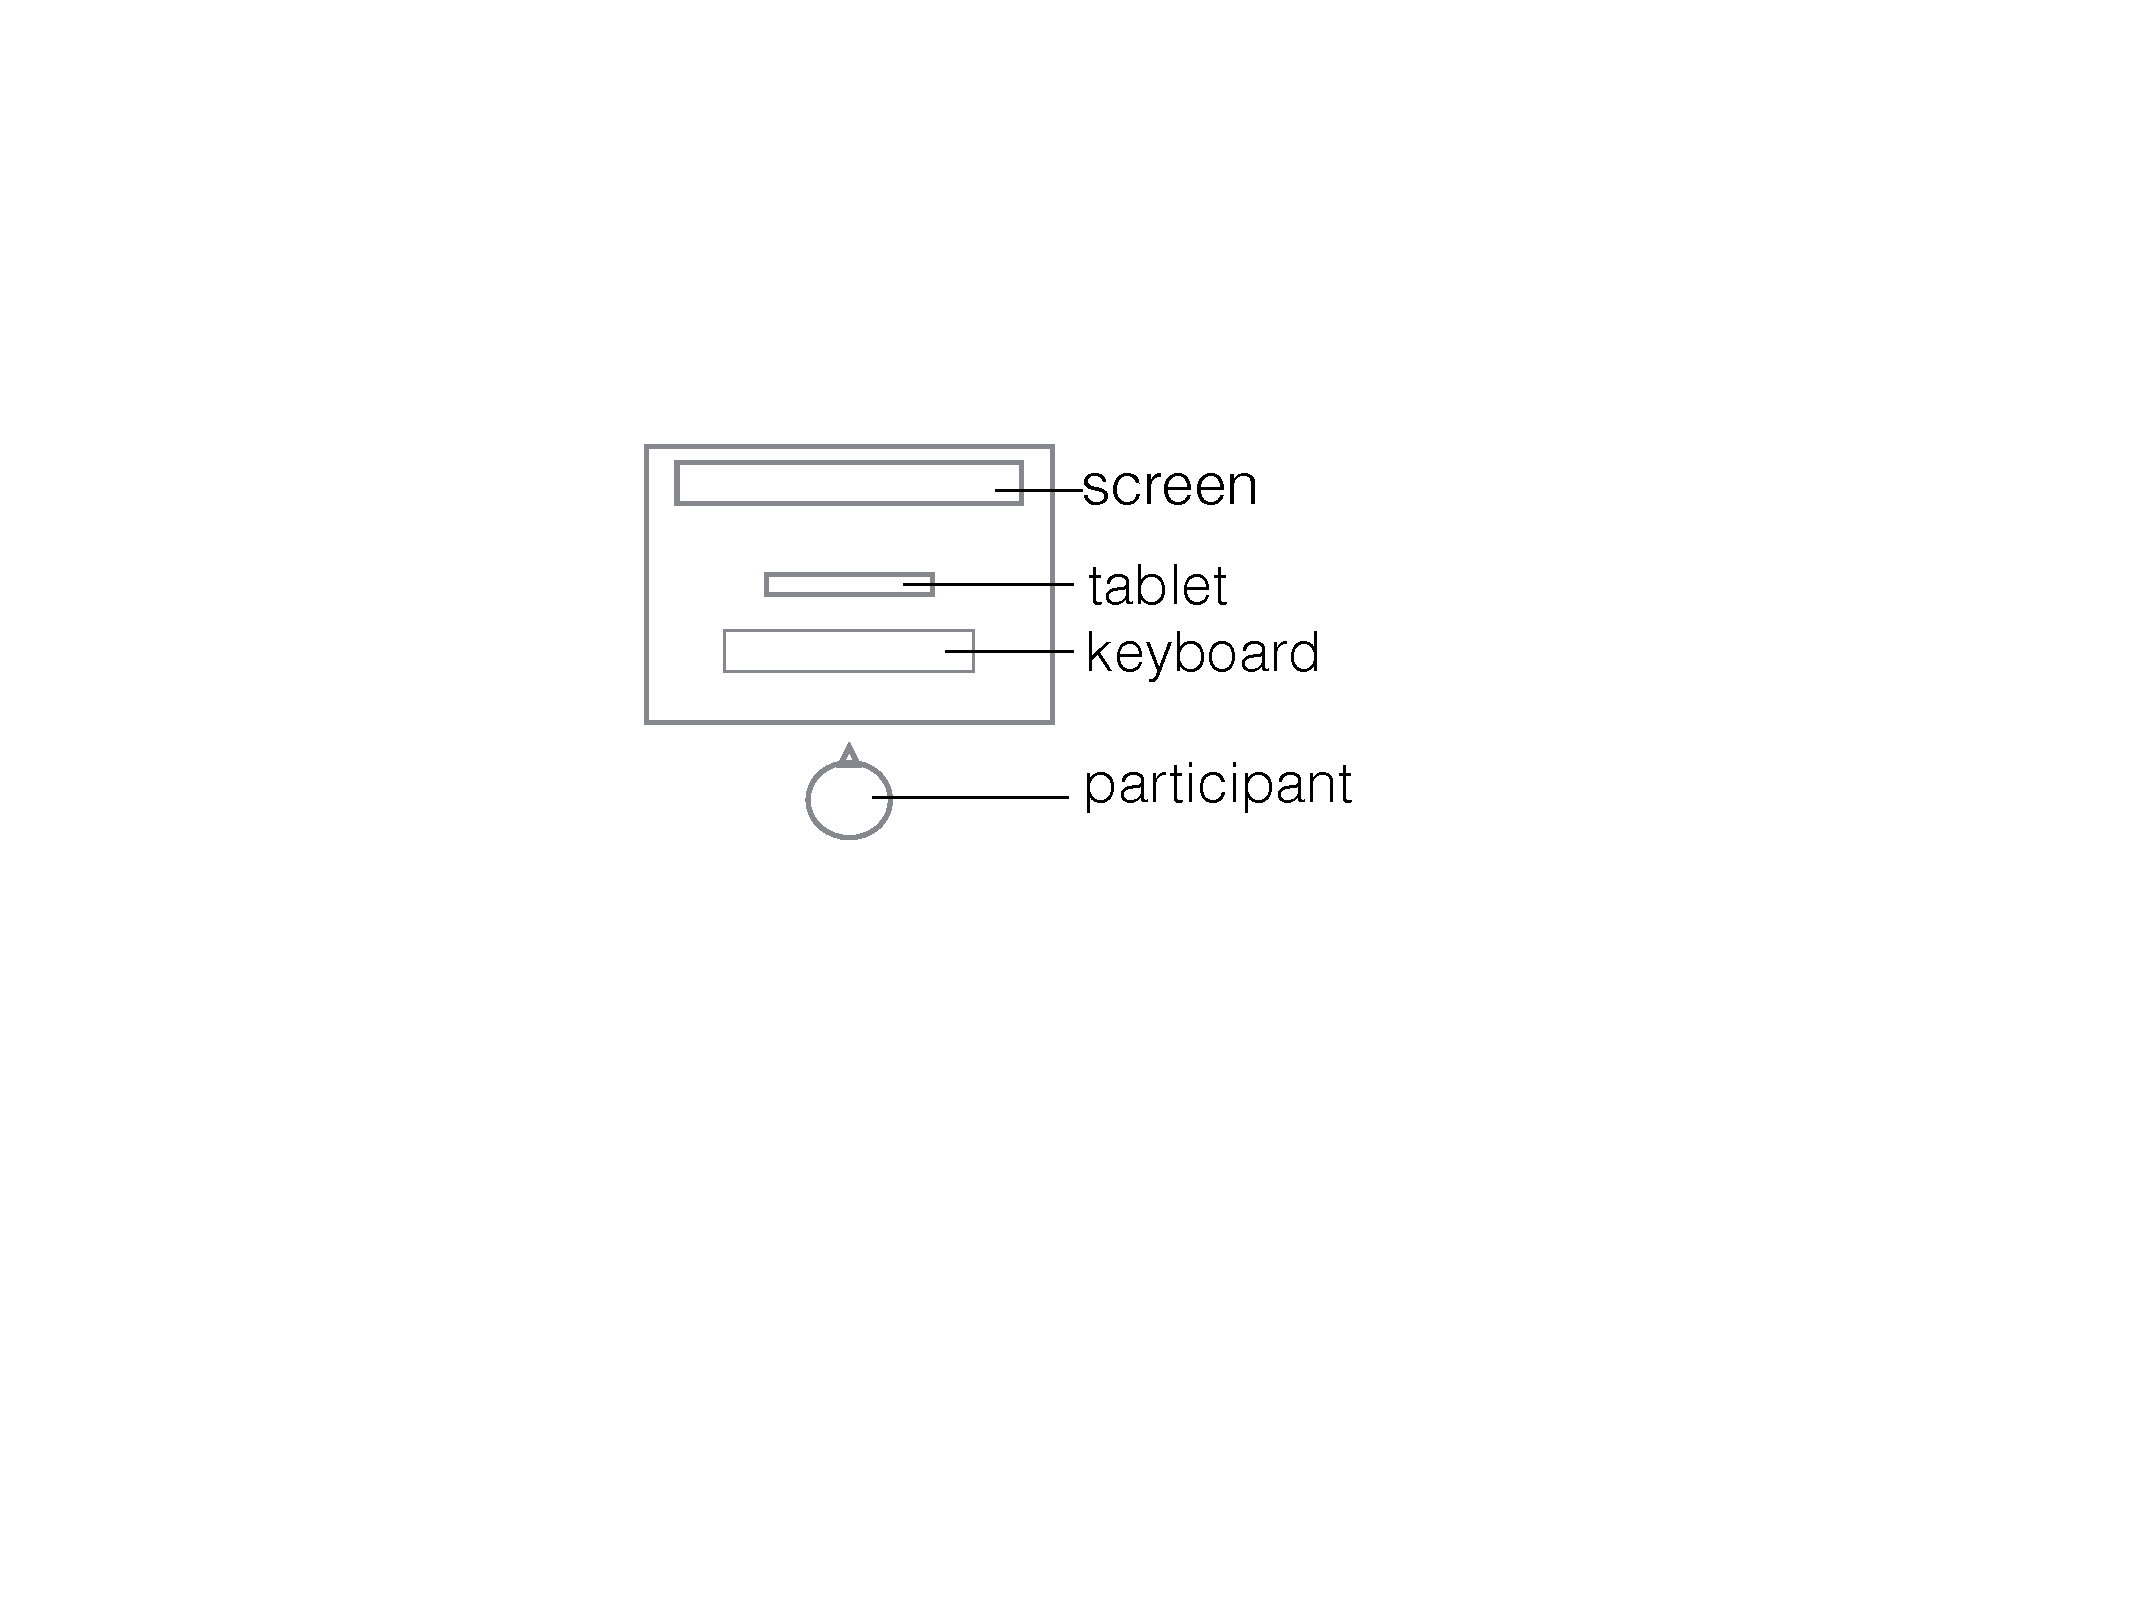
\includegraphics[width=0.5\textwidth]{figures/dataview.pdf}	
      \caption{Bird's eye view of the experiment: the participant sat at a table with a screen, tablet, and keboard in front of them. \label{fig:dataview}}
\end{figure}

The participant was told that she would interact with the system in three different phases, each for 4 minutes, and was instructed to accomplish as many tasks as possible in that time allotment. The participant was not told what the diffrent phases were, only that the system was somewhat different in each phase. The experiments described in Sections~\ref{section:exp1} and \ref{section:exp2} respectively describe and report a comparison first between the first and second phase (denoted as the \emph{endpointed} and \emph{incremental} variants of the system) and a comparison between the second and third phase (\emph{incremental} and \emph{incremental-adaptive} phases). Each of these phases are described below. Before the participant began Phase 1, they were able to try it out for up to 4 minutes (in Phase 1 settings) and ask questions about how it worked, allowing them to get used to the interface before the actual experiment began. After this trial phase, the experiment began.

\paragraph{Phase 1: Non-incremental} In this phase, the system did not appear to work incrementally; that is, the system only displayed tree updates after \asr\ endpointing (of 1.2 seconds, which is a resonable amount of time to expect a response from a commercial spoken \pa). The system displayed the ongoing \asr\ on the tablet as it was recognised (as is often done in commercial \pa s). The participant knew that the system fully understood the task when the displayed tree had no more unfilled branches (as in Figure~\ref{fig:filled})--as is the case in all phases. 

\paragraph{Phase 2: Incremental} In this phase, the system displayed the tree information incrementally as explained above. The \asr\ was no longer displayed; only the tree provided feedback in understanding. 

After Phase 2, a 10-question questionnaire was displayed on the screen for the participant to fill out comparing Phase 1 and Phase 2. For each question, they had the choice of \emph{Phase 1}, \emph{Phase 2}, \emph{Both}, and \emph{Neither}. (See appendix for full list of questions.) 

\paragraph{Phase 3: Incremental-adaptive} In this phase, the incremental system was again presented to the participant with an added user model that ``learned'' about the user. If the user saw a task more than once, the user model would predict that, if the user chose that task domain again (e.g., \emph{route}) then the system would automatically ask a clarification on the slots. If the user saw a task more than 3 times, the system skipped asking for clarifications and filled in the domain slots completely, requiring the user only to press the spacebar to confirm it was the correct one (i.e., to end the task). An example progression might be as follows: a participant is presented with the task \emph{route from Bielefeld to Berlin}, then the user would attempt to get the system to fill in the tree (i.e., slots) with those values. After some interaction in other domains, the user sees the same task again and here the user must only say ``yes'' for each slot to confirm the system's prediction. Later, if the task is presented a third time, the user would enter that domain (i.e, \emph{route}) and the two slots would already be filled. If later a new route task was presented (e.g., \emph{route from Bielefeld to Hamburg} the system would already have the slots filled for \texttt{from:Bielefeld}, \texttt{destination:Berlin}, but the user could backtrack by saying ``no, to Hamburg'' which would trigger the system to fill \texttt{destination:Hamburg}. Later interactions within the \emph{route} domain would ask for a clarification on the \emph{destination} slot since it has had several possible values given by the participant. 

After Phase 3, the participants were presented with another questionnaire on the screen to fill out with the same questions (plus two additional questions), this time comparing Phase 2 and Phase 3. For each question, they had the choice of \emph{Phase 2}, \emph{Phase 3}, \emph{Both}, and \emph{Neither}. At the end of the three phases and questoinnaries, the participants were given a final questionnaire to fill out by hand on their general impressions of the systems. 

We recruited 14 participants to participate in the evaluation. We used the Mint tools data collection framework described in \newcite{kousidis2012evaluating} to log the interactions. Due to some technical issues, one of the participants did not log interactions, we collected data from 13 participants, post-Phase 2 questionnaires from 12 participants,  post-Phase 3 questionnaires from all 14 participants, and general questoinnaires from all 14 participants. In the experiments that follow, we report object and subjective measures to determine the settings that produced superior results.

\paragraph{Metrics} We report the subjective results of the participant questionnaires. We only report those items that were statistically significant (see Appendix for a list of the questions). We further report objective measures for each system variant: total tasks, fully correct frames, average frame fscore, and average time elapsed (averages are taken over all participants for each variant; we only used the 10 participants who fully interacted with all three phases). Discussion of the two experiments is left to the end of this section.

\subsection{Experiment 1: Endpointed vs. Incremental}
\label{section:exp1}

In this section we report the results of the evaluation between the \emph{endpointed} (i.e., non-incremental; Phase 1) vs the incremental (Phase 2) variants of our system.

\subsection{Subjective Evaluation} We applied a multinomial test of significance to the results, treating all four possible answers as equally likely (with Bonferroni correction of 10). The question \emph{The interface useful and easy to understand} with the answer of \emph{Both} was significant ($ \chi^2 $ (4, N = 12) = 9.0, p $<$ .005), as was \emph{The assistant was easy and intuitive to use} also with the answer \emph{Both} ($ \chi^2 $ (4, N = 12) = 9.0, p $<$ .005). The question \emph{I always understood what the system wanted from me} was also answered \emph{Both} significanly more times than other answers ($ \chi^2 $ (4, N = 14) = 9.0, p $<$ .005), similarly for the item \emph{It was sometimes unclear to me if the assistant understood me} with the answer of \emph{Both} ($ \chi^2 $ (4, N = 12) = 10.0, p $<$ .005). 

These responses tell us that though the participants did not report preference for either system variant, they reported a general positive impression of the interface (in both variants). This is a nice result; the \ui\ could be used in a traditional, non-incremental way or in an incremental way and could be useful to users. 

\subsection{Objective Evaluation}  The \emph{endpointed} (Phase 1) and \emph{incremental} (Phase 2) columns in Table~\ref{tab:objscores} show the results of the objective evaluation. Though the average time per task and fscore for the endpointed variant are better than those of the incremental version, the total number of tasks for the incremental variant was higher, as was the number of fully correct frames (though only by a count of 2). 


\begin{table}
 \begin{tabular}{|r|c|c|c|}
\hline
                     & \textbf{endpointed} & \textbf{incremental} & \textbf{adaptive} \\
\hline
\textbf{tasks} & 105 & 122 & 124  \\
\textbf{frames} & 46 & 46 & 59 \\
\textbf{fscore} & 0.81 & 0.74 & 0.80 \\
\textbf{time} & 19.1 & 19.6 & 19.5 \\
 \hline
\end{tabular}
\caption{Objective measures for Experiments 1 \& 2: count of completed tasks, number of fully correct frames, average fscore (over all participants), and average elapsed time per task (over all participants).}
\label{tab:objscores}
\end{table}

\subsection{Experiment 2: Incremental vs. Incremental-Adaptive}
\label{section:exp2}

\subsection{Subjective Evaluation} The questionnaire comparing Phase 2 (incremental) and Phase 3 (incremental-adaptive) contained 12 questions, each with a choice of \emph{Phase 2}, \emph{Phase 3}, \emph{Both}, and \emph{Neither}.  We applied a multinomial test of significance to the results, treating all four possible answers as equally likely (with Bonferroni correction of 12). The question \emph{The interface useful and easy to understand} was answered \emph{Both} significantly more than other answers  ($ \chi^2 $ (4, N = 14) = 10.0, p $<$ .0042), The item \emph{I had the feeling that the assistant attempted to learn about me} was answered significantly with \emph{Neither} ($ \chi^2 $ (4, N = 14) = 8.0, p $<$ .0042), though the only other marked answer was \emph{Phase 3} (6 times), showing that either the participants didn't notice that either phase was attempting to apply a user model at all, but if they did notice, only Phase 3 was marked. All other questions were not significant.

Here again we see that there is a general positive impression of the \ui\ under all conditions. If anyone noticed that a system variant was attempting to learn a user model at all, they noticed that it was in Phase 3, as expected. 

\subsection{Objective Evaluation} The \emph{incremental} (Phase 2) and \emph{adaptive} (Phase 3) columns in Table~\ref{tab:objscores} show the results for the object evaluation for this experiment. Here, there is a clear difference between the two variants, with the adaptive showing more completed tasks, more fully correct frames, a higher fscore (all three possibly due to the fact that frames were potentially pre-filled), though the elapsed amount of time for each task was overall slightly higher. 

\subsection{Discussion}

While the questionnaires don't express any preference for a particular system variant, the overall impression of the \ui\ was positive. The objective measures show that there are gains to be made when the system signals understanding at a more fine-grained interval than at the utterance level, due to the higher number of completed tasks. There are further gains to be made when the system applies even simple notions of user modeling (i.e., adaptivity) by attempting to predict what the user might want to do given a chosen domain; allowing the system to fill the frames decreases the possibility of user error, allowing the system to successfully complete more tasks in a shorter amount of time. 

The final open-ended questionnaire sheds additional light on participants' experiences with our system(s). Most of the complaints (i.e., suggestions for improvement) revolved around problems with \asr, not the system itself (e.g., in Phase 1 the \asr\ was displayed and the wrong words were recognised; also that the \asr\ reponses were too slow). Two participants suggested an alternative ability to add ``free input'' as to override the \asr\ with hand-typed input (or select alternatives from the list with a scroll and touch interface in addition to the speech interface). Two participants suggested that the system be more responsive (i.e., more clearly show that the system was working even if the \ui\ did not change) and give more feedback (i.e., backchannels) more often. For those participants that expressed preference to the non-incremental system (Phase 1), none of them had used a speech-based \pa\ before, whereas those that expressed preference to the incremental versions (Phases 2 and 3) have used speech-based \pa s before, and use them regularly. We conjecture that people without experience like to know how well the \asr\ is working and equate understanding with \asr, whereas those that are more familiar with \pa s know that perfect \asr\ doesn't necessarily translate to perfect understanding--hence the need for an interface like the one presented here. 

\section{Conclusion \& Future Work}

Given the subjective and object results and analysis, we conclude that an intuitive presentation that signals a system's ongoing understanding benefits end users who perform simple tasks might be performed by a \pa. The presenteation that we provided, using a right-branching tree, worked well; indeed, the participants who used it found it intiutive and easy to understand. There are gains to be made when the system signals understanding at finer-grained levels than just at the end of a pre-formulated utterance. There are further gains to be made when a \pa\ attempts to learn (even a rudimentary) user model to predict what the user might want to do next. 

For future work, we intend to provide simple authoring tools for the system to make building simple \pa s using our \ui\ easy. We want to improve the \nlu\ and scale to larger domains. We also plan on implementing this as a standalone application that could be run on a mobile device, which could actually perform the tasks.


\section*{Appendix}

The following questions were asked on both questoinnaries following Phase 2 and Phase 3 (comparing the two most latest used system versions):
\begin{itemize}
 \item The interface useful and easy to understand.
 \item The assistant was easy and intuitive to use.
 \item The assistant understaood what I wanted to say.
 \item I always understood what the system wanted from me. 
 \item The assistant made many mistakes. 
 \item The assistant did not respond while I spoke.
 \item It was sometimes unclear to me if the assistant understood me. 
 \item The assistant responde while I spoke. 
 \item The assistant sometimes did things that I did not expect.
 \item When the assistant made mistakes, it was easy for me to correct them. 
\end{itemize}

In addition to the above 10 questions, the following were also asked on the questionnaire following Phase 3:
\begin{itemize}
 \item I had the feeling that the assistant attempted to learn about me.
 \item I had the feeling that the asssitant made incorrect guesses. 
\end{itemize}


The following questions were used on the general questoinnaire (as translated into English):
\begin{itemize}
 \item I regularly use peronal assistants such as Siri, Corana, Google now or Amazon Echo: Yes/No
 \item I have never used a speech-based personal assistant: Yes/No
 \item What was your general impression of our personal assistants?
 \item Would you use one of these assistants on a smartphone or tablet if it were available? If yes, which one?
 \item Do you have suggestions that you think would help us improve our assistants?
 \item If you have used other speech-based interfaces before, do you prefer this interface?
\end{itemize}


\bibliographystyle{acl2016}
\bibliography{refs}

\end{document}

